%=========================================================================
\chapter{The RdRand instruction}  \label{chap:rdrand-instruction}
First public information about RdRand came somewhen during year 2011\cite{IntelRdRandFindAbout}, a year before the CPUs with it were released and Intel itself send patches to add support into Linux in summer of the same year\cite{KernelRdRand}. Later, RdRand was added between Linux entropy sources for {\tt /dev/[u]random}.\TODO{Find discussion}% TODO find discussion
According to known information\cite{TheodoreTsoNSA}, Intel tried to have {\tt /dev/[u]random} rely only on their instruction, but that was denied. 

We weren't able to find any relevant data about usage of RdRand in Windows kernel, probably because all such negotiations happened behind closed doors. In user space, there is no difference between Linux and Windows; when it is possible to call the instruction, user space applications can use it. 

After disclosure of extends of NSA spying activities by Edward Snowden in summer of 2013\cite{GuardianNSA}\cite{DailymailNSA}, a petition for removing RdRand from Linux entropy sources was created\cite{PetitionRdRand}. Although supported by just 8 signatures, it got wide attention on information-technology aimed news pages and magazines, like Slashdot.org\cite{PetitionRdRandSlashdot}. The petition was closed after Linus Torvalds responds with scorn:

\begin{quote} ...

Short answer: we actually know what we are doing. You don't.

Long answer: we use rdrand as \_one\_ of many inputs into the random pool, and we use it as a way to \_improve\_ that random pool. So even if rdrand were to be back-doored by the NSA, our use of rdrand actually improves the quality of the random numbers you get from {\tt /dev/random}.

...
\end{quote}


\section{Intel Secure Key} \label{sec:intel-secure-key}
The Intel Secure Key (ISK) uses cascade construction, combining a HW RNG with CSPRNG into one sealed block on CPU, which is compliant with many security standards, including NIST SP800-90, FIPS-140-2, and ANSI X9.82\cite{IntelDRNGGuide}. Although it is impossible to audit it, there was found no evidence of low entropy or anything that would deny the security standards compliance - neither with tests in chapter \nameref{chap:statistical-testing}, nor any other tests anyone else did\footnote{I assume that such revelation would become quickly known and broadly discussed.}.

\section{Physical implementation}
One important thing about ISK, that has big impact on performance, but also price of that solution is, that there is only one unit on a die and the unit should be the same on all CPUs.\TODO{quote it} % TODO quote it
Because all processing units (PU)\footnote{Two physical cores with hyper-threading counts as four PU.} on one die share the RNG, one thread reading random numbers from it can never be faster than $Total speed  \frac{1}{PUs}$. The effect of this is that the performance is perfectly scalable (see \nameref{chap:performance} chapter), and price of the CPU is less affected.

Each ISK unit consists three basic parts: A hardware entropy source, a conditioner and a PRNG\cite{IntelDRNGGuide}.
\begin{figure}[h!]
  \centering
 \includegraphics[width = 10cm,keepaspectratio]{fig/ISK-scheme.pdf} % Or .pdf
%\includegraphics[width=10cm,keepaspectratio]{fig/ISK-scheme}
\caption{An Intel Secure Key unit}
\label{fig:ISK-unit}
\end{figure}

\section{Existing usages} 
Kernel, openssl
\section{Possible usages}

%========================================================================= 
